\documentclass[urlcolor=blue,dvipsnames]{beamer}

\usepackage[utf8]{inputenc}
\usepackage{fancybox,fancyvrb}
\usepackage{environ,xspace}
\usepackage{tikz}
\hypersetup{colorlinks,linkcolor=,urlcolor=cyan}

\beamertemplatenavigationsymbolsempty
\setbeamertemplate{footline}[frame number]
\usetheme{Pittsburgh}

\newcommand\enumnum[1]{{\renewcommand{\insertenumlabel}{#1}%
      \usebeamertemplate{enumerate item} \,}}

\newcommand{\grad}{\nabla}
\newcommand{\ih}{\boldsymbol{\hat{\textbf{\i}}}}
\newcommand{\jh}{\boldsymbol{\hat{\textbf{\j}}}}
\newcommand{\vF}{\boldsymbol{\vec{\textbf{F}}}}
\newcommand{\Matlab}{\textsc{Matlab}\xspace}
\newcommand{\Octave}{\textsc{Octave}\xspace}


\title{5.3 Nonlinear models \\ (with some 4.10 material too)}

\subtitle{a lesson for MATH F302 Differential Equations}

\author{Ed Bueler, Dept.~of Mathematics and Statistics, UAF}

\date{\tiny \today}


\begin{document}
\setbeamertemplate{itemize item}{$\bullet$}
\setbeamertemplate{itemize subitem}{$\circ$}


\begin{frame}
\titlepage

\centerline{\tiny for textbook: \, D. Zill, \emph{A First Course in Differential Equations with Modeling Applications}, 11th ed.}
%\color{green!40!blue}
\end{frame}


\begin{frame}{outline}

examples of nonlinear 2nd-order differential equations (DEs):

\begin{itemize}
\item pendulum (\S 5.3)
\item using a numerical solver in \Matlab/\Octave (see \S4.10)
\item hard and soft springs (\S 5.3)
\item non-constant gravity: from earth to high orbit (\S 5.3)
\item dependent variable missing (\S 4.10)
\end{itemize}
\end{frame}


\begin{frame}{nonlinear pendulum}

\begin{columns}
\begin{column}{0.7\textwidth}
\begin{itemize}
\item suppose a pendulum oscillates (swings back and forth) without resistance
\item if you believe my \S5.1 slides then it must be modeled by a 2nd-order linear DE
     \begin{itemize}
     \item this is true for small oscillations 
     \item for bigger oscillations (more than 20$^\circ$?) a nonlinear model is more accurate
     \end{itemize}
\item the DE which comes from the diagram:
    $$m \ell \frac{d^2\theta}{dt^2} = - mg \sin\theta$$

\vspace{-2mm}
     \begin{itemize}
     \item you are not responsible for the derivation
     \item \dots but $s=\ell \theta$ is arclength, so $\ell \frac{d^2\theta}{dt^2}$ is acceleration, and only the tangential force is relevant
     \end{itemize}
\end{itemize}
\end{column}
\begin{column}{0.3\textwidth}
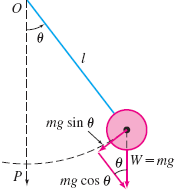
\includegraphics[width=\textwidth]{figs/pendulum}
\end{column}
\end{columns}
\end{frame}


\begin{frame}{linear small angle model}

\begin{itemize}
\item divide by $m\ell$ and move term: \quad $\displaystyle \frac{d^2\theta}{dt^2} + \frac{g}{\ell} \sin\theta = 0$
\item if $\displaystyle \omega = \sqrt{\frac{g}{\ell}}$ then \, $\displaystyle \boxed{\frac{d^2\theta}{dt^2} + \omega^2 \sin\theta = 0}$ \, for any angle
\item recall $\sin\theta \approx \theta$ for small $\theta$ because $\sin z = z - \frac{z^3}{3!} + \frac{z^5}{5!} - \dots$
\item a \emph{small angle model}:
    $$\boxed{\frac{d^2\theta}{dt^2} + \omega^2 \theta = 0} \hspace{20mm}$$
    \begin{itemize}
    \item solution: $\theta(t) = c_1 \cos(\omega t) + c_2 \sin(\omega t)$
    \end{itemize}
\end{itemize}

\vspace{-30mm}
\hfill 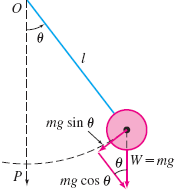
\includegraphics[width=0.25\textwidth]{figs/pendulum}

\end{frame}


\begin{frame}{nonlinear versus linear}

\begin{center}
\begin{tabular}{c|c}
nonlinear: any angles & linearized: small angles \\ \hline
$\Huge \strut$ $\displaystyle {\color{Green} \frac{d^2\theta}{dt^2} + \omega^2 \sin\theta = 0}$ & $\displaystyle \frac{d^2\theta}{dt^2} + \omega^2 \theta = 0$ \\ \hline
$\huge \strut$ solution? & $\theta(t) = c_1 \cos(\omega t) + c_2 \sin(\omega t)$
\end{tabular}
\end{center}

\begin{itemize}
\item note $\omega = \sqrt{g/\ell\,}$ in both DEs
\item we don't know how to solve a nonlinear DE like {\color{Green} the pendulum}
    \begin{itemize}
    \item $\theta=e^{rt}$ is not a solution for any $r$, whether real or complex
    \item the term ``${\color{Green} \sin\theta}$'' is not linear
    \item using the concept of \emph{energy} makes progress (Mini-Project 3)
    \item numerical approximations? $\large \strut$
       \begin{itemize}
       \item Euler's method? \dots inefficient but would work
       \item next: using a ``black box'' solver in \Matlab/\Octave
       \end{itemize}
    \end{itemize}
\end{itemize}
\end{frame}


\begin{frame}{X}

\begin{itemize}
\item X
\end{itemize}
\end{frame}


\begin{frame}{X}

\begin{itemize}
\item X
\end{itemize}
\end{frame}


\begin{frame}{X}

\begin{itemize}
\item X
\end{itemize}
\end{frame}


\begin{frame}{expectations}

\begin{itemize}
\item just watching this video is \emph{not} enough!
     \begin{itemize}
     \item see ``found online'' videos at

     \centerline{\href{https://bueler.github.io/math302/week8.html}{\tt \color{cyan} bueler.github.io/math302/week8.html}}
     \item \emph{read} section 4.10 in the textbook
         \begin{itemize}
         \item skip the ``Use of Taylor series'' material \dots we'll get to it later
         \end{itemize}
     \item \emph{read} section 5.3 in the textbook
         \begin{itemize}
         \item you can safely skip the material on ``Telephone wires'' (a boundary value problem \dots not in Math 302)
         \end{itemize}
     \item \emph{do} the WebAssign exercises for section 5.3, which include some problems from 4.10
     \end{itemize}
\end{itemize}
\end{frame}

\end{document}

